
\ifx\isEmbedded\undefined

\documentclass[12pt,a4paper]{report}
\usepackage[bottom=2.5cm,left=2.0in,right=2.5cm]{geometry}

% FONT RELATED
\usepackage{times} %Move to times font
\usepackage[labelfont=bf,textfont=it]{caption}

% LINKS, PAGE OF CONTENT, REF AND CROSS-REF, HEADERS/FOOTERS
\usepackage{footmisc}
\usepackage{hyperref}
\usepackage{bookmark}
\usepackage{fancyhdr}
%\usepackage{nameref}

% FIGURES, GRAPHICS, TABLES
\usepackage{graphicx}
\usepackage{parskip}
\usepackage{tocloft}
\usepackage{array}
\renewcommand{\cftfigfont}{Figure }
\renewcommand{\cfttabfont}{Table }
\usepackage{longtable}

%\newlength{\mylen}
%\renewcommand{\cftfigpresnum}{\figurename\enspace}
%\renewcommand{\cftfigaftersnum}{:}
%\settowidth{\mylen}{\cftfigpresnum\cftfigaftersnum}
%\addtolength{\cftfignumwidth}{\mylen}






%\usepackage{subfigure}
\usepackage{wrapfig}
\usepackage{caption}
\usepackage{subcaption}


% COLOURS, TEXT AND FORMATTING
%\usepackage[left=2.0in,right=0.5in]{geometry}

\usepackage{array}
\usepackage{color}
\usepackage{setspace}
\usepackage{longtable}
\usepackage{multirow}


% ADVANCED MATHS, PSEUDO-CODE
\usepackage{amsmath}
\usepackage{amsfonts}
\usepackage{alltt}
%\usepackage{algorithm2e}
\usepackage{algorithmicx}
\usepackage{algorithm}
\usepackage{algpascal}
\usepackage{algc}
\usepackage{algcompatible}
\usepackage{algpseudocode}
\usepackage{linegoal}

% BIBLIOGRAPHY
\usepackage{natbib}
%\usepackage[authoryear]{natbib}
%\usepackage{harvardnat}
\bibpunct{(}{)}{;}{a}{}{,}
%\usepackage{bibentry}
%\nobibliography*



% LINE NUMBERS
%\usepackage{lineno}
%\linenumbers

% USE IN DISSERTATION:

% MARGINS
%\setlength{\oddsidemargin}{2.0in}
%\setlength{\evensidemargin}{0.5in}
%\setlength\headsep{2.5in}

% TEXT
\setlength\textheight{9.5in}
\setlength\textwidth{5.1in}

% indent at each new paragraph
\setlength\parindent{1.0cm}
%\setlength\parindent{0.5cm}

%\setlength{\parskip}{10.5ex}

\setlength\topmargin{-0.2in}

% 1.5 spacing:
\renewcommand{\baselinestretch}{1.5}
%\renewcommand{\baselinestretch}{1.3}
%\fontsize{15}{15}\selectfont

% USE IN REPORT:

%\setlength\oddsidemargin{1cm}
%\setlength\evensidemargin{0.3in}
%%\setlength\headsep{2.5in}
%
\setlength\textheight{9.0in}
%\setlength\textwidth{5.5in}
%
%% indent at each new paragrapg
%\setlength\parindent{0.5cm}
%
%%\setlength{\parskip}{10.5ex}
%
%\setlength\topmargin{-0.2in}

%\newcommand{\HRule}{\rule{\linewidth}{0.5mm}}
\newcommand{\HRule}{\rule{\linewidth}{0.0mm}}

% Color definitions (RGB model)
\definecolor{color-comment}{rgb}{0.1, 0.4, 0.1}
\definecolor{color-variable}{rgb}{0.000,0.000,0.616}
\definecolor{color-question}{rgb}{0.4, 0.0, 0.0}
\definecolor{color-new}{rgb}{0.2, 0.4, 0.8}

\newcommand*{\Let}[2]{\State #1 $\gets$
\parbox[t]{\linegoal}{#2\strut}}

\newcommand*{\LongState}[1]{\State
\parbox[t]{\linegoal}{#1\strut}}

\graphicspath{{../images/}}
\begin{document}
%\maketitle
\fi


%**************************************************************************
%**************************************************************************
\chapter{Literature Review}
\label{cha:literature_review}

Clothing is one of the most distinctive features of human being which differs us from other creatures. The history of cloth can be traced back to 107,000 years ago\Citep{Kittler2003, Toups2011}. During the development of cloth, the basic function of cloth remains, which is to provide protection to the wearer from environment. Cloth also performs a wide range of cultural and social functions which expresses the personality, occupation, sexual differentiation, and social status of the wearer \Citep{Harms1938}.

In the world of today, with high speed development of computer hardware and computer graphic techniques, realistic virtual character has been wildly used in film, TV and game productions. Apart from body motions and facial expressions, same as in reality, cloth plays a very important role in acting. In order to achieve high visual realism, many techniques have been developed in areas such as motion capture, muscle simulation, or skin deformation, etc. However, in computer animation, virtual clothing which involves both textile engineering knowledge and artistic expertise, is considered as a challenging task. Especially for cloth modelling, it still requires large amount of manual operation and it is a very time-consuming task in the animation production. 

%The cloth making techniques have been developed for hundreds years, a well developed cloth production pipeline is widely used in today's cloth manufacturing. 

Cloth pattern is the most common cloth design representation in the fashion industry. This thesis presents an pattern based cloth modelling method for animation artist which improves efficiency and reduce tediousness of current pattern based cloth modelling techniques by automating the pattern adjusting processes requires deep tailoring knowledges. This chapter firstly presents a general overview of the cloth production procedure in fashion industry. In order to make cloth that fits the target character, the measurements of character is crucial, therefore, a detailed introduction of research achievements in anthropometry study is also presented. After that, the state of the art virtual clothing techniques in both fashion industry and computer animation are introduced. Because the measuring method presented in this thesis utilises geodesic for length measurements extraction and uses genetic algorithm to adjust cloth patterns automatically, therefore, a brief review on geodesic algorithm and genetic algorithm finally is presented.


%--------------------------------------------------------------------------
\section{Patternmaking in Fashion Design}

The process of constructing a complete cloth consists of several interdependent steps. Each step heavily affects the appearance and fit of the garment. Within these steps, patternmaking settles among the earliest few steps in the construction of a complete cloth. It is a highly skilled craft that has evolved over the centuries. 

In ancient Roman period, producing textile materials was a laborious process. Fabric was weaved using primitive looms entirely by hand. Therefore, fabric was a very expensive commodity and it was an important symbol for the social status of the wearer. In terms of cloth structure at that time, cloth was mainly made by a set of uncut, rectangular shaped fabric pieces in order to minimize waste  \Citep{Caroline1996}. 

\begin{figure}[ht]
    \centering
	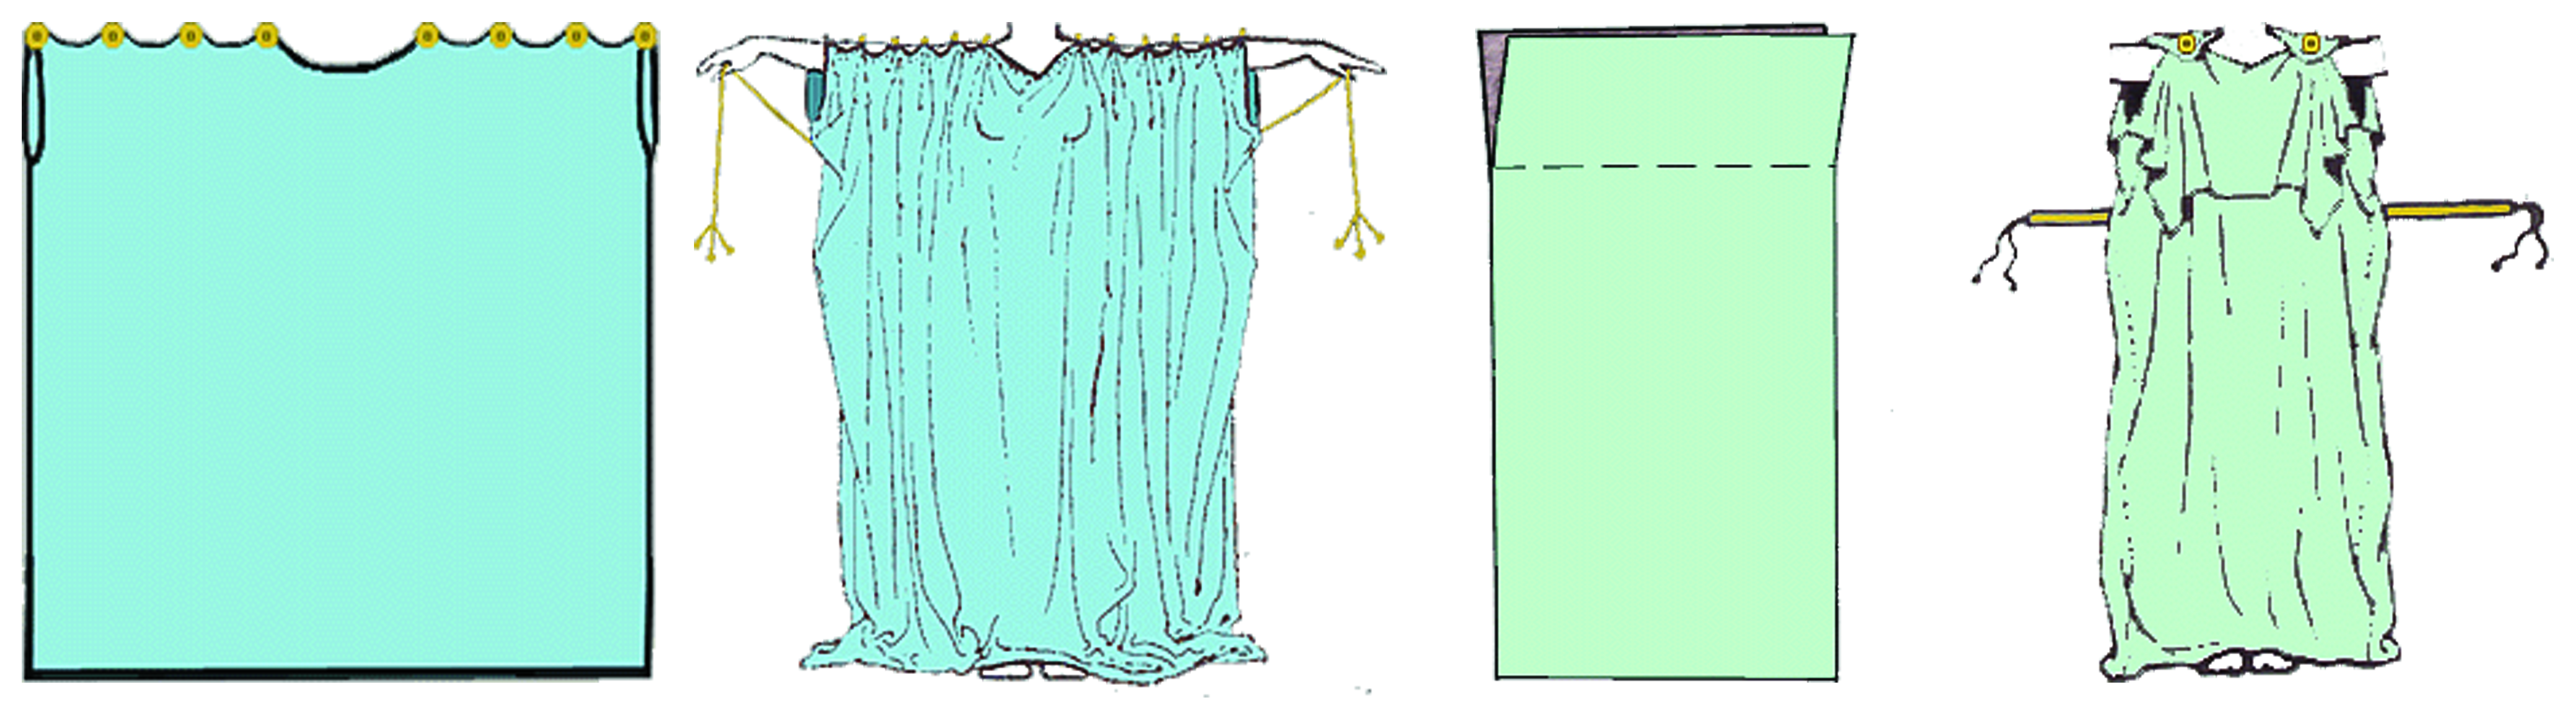
\includegraphics[width=\columnwidth]{../images/ancient_roman_cloth}\\[1cm]
    \caption{The peplos(left) and the chiton(right) was the common cloth wear by woman in ancient Roman \Citep{McManus2003}.}
    \label{figure:fig3}
\end{figure}

In the 15th century, the seminal art of patternmaking began. The fabric was carefully trimmed to fit the contour of body \Citep{macdonald2009principles}. The foundation of the modern fashion design was built since then. Before the industrial revolution, patternmaking is a highly respected art. During that time, tailors choicely worked with the measurements taken from their costumer to handmade cloth patterns. Only the high society are able to afford tailor made cloth. During the industrial revolution, the standardization of cloth pattern has become essential to the popularization of massive produced cloth. However, initial attempts to create standardized cloth pattern resulted in a little detailed cloth that is poorly fitted. After large amount of experimentations and standardization of sizing regulation, patternmaking has successfully transferred from customization to standardization\Citep{macdonald2009principles}. During that time, cloth patterns are made into one size and tailor had to grade cloth pattern to the size that wearer was needed. Because pattern-grading requires lots of tailoring expertise and experiences, cloth pattern was not widely accepted in home sewing. At the end of 19th century, Butterick introduced revolutionary graded cloth patterns\Citep{butterick1994butterick} to the world. The effects of this idea were significant as it opens up the market of home sewing to the general public. Butterick's pattern not only made dressmaking much easier, but also pushed fashion from high class into general public all over the world. During the WWII,  with the help of the development of anthropometry, sizing chart was introduced based on anthropometric data. The use of sizing chart in graded patterns production have made it fit the general public better than before. Nowaday, after nearly a century, graded patterns has been widely accepted by today's fashion industry\Citep{noke1987history, rosen2004patternmaking}. 

Based on different target customers, today's patternmaking techniques can be classified into two general categorises, patternmaking for massive production\Citep{nugent2008computerized, shoben1987pattern, stecker1996fashion, 2007hand}, and patternmaking for custom tailoring\Citep{margolis1964complete, cabrera1983classic, 2011practical}. Patternmeking for massive production mainly focus at the ease of pattern distribution and standardization. This type of patternmaking techniques grade patterns into different predetermined size in order to fit the most of customers. In custom tailoring, patterns are distributed as an one size design concept, the final cloth requires experienced tailor to fine tune the size and shape of cloth patterns based on measurements taken from customer to create a fit cloth. 

%The research presented in this thesis brings the idea of custom tailoring into the construction of virtual cloth. Cloth are created from cloth patterns that are adjusted based on the measurements of a character. This approach allows a cloth design to be fitted onto any character. 


%--------------------------------------------------------------------------
\section{Anthropometry}

Fit is a essential requirement for clothing that directly determines the functionality of a cloth. In order to achieve fit, measurements of the wearer's body need to be acquired. Anthropometry is a branch of human science that studies human body size, shape, mobility, flexibility and strength \Citep{gupta2014anthropometry}. Human body dimension, as ours personality, is largely varied among the population. Many user-centred applications require understanding of the variability of human body dimension. Especially for garment industry, as cloth is an object that its functionality is determined by its coverage and sealability. Both the coverage and the sealability need to be ensured by obtaining wearer's body measurements. This section debriefs the research achievements in anthropometry and introduces several methods for anthropometry data acquisitions. 

Human physical stature was the first topic which was studied systematically in anthropometry. Its history can be traced back to 18th century \Citep{tanner_history_1981}. However, the recognition of human body proportion is far earlier than 18th century. In ancient Egypt, a modular grid was often used for the preparation of human figure painting by tome painters \Citep{pheasant2006bodyspace}. This modular grid consists of 18 units from the crown of skull to feet. Figure \ref{figure:fig1} demonstrates three ancient Egyptian figures that have 18:11 relationship between the height of hairline to the navel \Citep{robins1994proportion}. The separation of modular grid provides a consistent guideline upon which a figure's proportions could be based on.

\begin{figure}[ht]
    \centering
	\includegraphics[width=\columnwidth]{../images/threefigures}\\[1cm]
	%\includegraphics[width=0.3\textwidth]{../images/bu_logo}\\[1cm]
    \caption{Body proportion in ancient Egypt }
    \label{figure:fig1}
\end{figure}

This modular system which was initially used as a drawing standard is still remaining in use today. The most detailed system of human proportions that today's anthropometry researches built on is from the Roman architectural theorist Vitruvius in 15 B.C\Citep{selin2008encyclopaedia}. His theory of human proportions is well known as the ``well-shaped man'' \Citep{Rudolf1955}, in which the height of the human stature is  equal to the arm span. Vitruvius also employs this human proportion as a fundamental principle in his building design as he claims that ``No temple can have a rational composition without symmetry and proportion, that is, if it has not an exact calculation of members like a well-shaped man''  \Citep{pollio1914ten, Marcus2002}.

The most recognized visualization of Vitruvius's human proportion is the drawing created by Leonardo da Vinci \Citep{stemp2006secret}. This piece is accompanied by nodes that are based on the theory of human body proportion developed by Vitruvius. It depicts a male figure in two superimposed postures that the arms and legs of a male person are circumscribed by a cycle and a square respectively. After this piece was created, the theory of human proportion had become bound up with the ``Golden ratio''. ``Golden ratio'' refers to the umbilicus divides of the stature of a male person in standing posture in golden section. Such that the ratio of the greater part of the stature to the whole body is equal to that of the lesser part to the greater part \Citep{stemp2006secret}.

\begin{figure}[H]
    \centering
	\includegraphics[width=0.48\columnwidth]{../images/Da_Vinci}\\[1cm]
    \caption[The Vitruvian Man]{The Vitruvian Man created by Leonardo da Vinci in 1490 \Citep{stemp2006secret}}
    \label{figure:fig2}
\end{figure}

However, the study carried out by Vitruvius was based on Roman population in 15 B.C. In the past two hundred years, anthropometry has shown that span exceeds height in 59-78\% of normal adult white men \Citep{Schott19921518}. Studies on anthropometry was not systematically carried out until 1870's. A Belgian mathematician who named Quetelet published a statistical analysis of the chest sizes of 5000 Scottish soldiers \Citep{quetelet2011anthropométrie}. This was the birth of the science of anthropometry. After that, in a very long time, anthropometric data was mainly used for taxonomic or physiological studies. The development of this science accelerated during WWII which was powered by aircraft industry due to the need of designing better aircraft cockpits. 

The measurements involved in modern anthropometry varies from field to field. In general, six measurements are used to describe a human stature, these six measurements are shown in Table \ref{table:tab4}.

%\setlength{\tabcolsep}{4pt}
\begin{table}[H]
        \centering
        %\begin{tabular}{|m{1.1cm}|m{0.8cm}|m{1.2cm}|m{1.2cm}|m{1.2cm}|m{1.2cm}|}
        \begin{tabular}{|l|m{9cm}|l|}
        \hline
        Height & Point-to-point vertical measurement\\
        \hline
        Breadth & Point-to-point horizontal measurement running across the body or segment\\
        \hline
		Depth & Point-to-point horizontal measurement running fore-and-aft along the body\\
		\hline
		Curvature & Ppoint-to-point measurement following a contour\\
		\hline
		Circumference &  Closed measurement that follows a body contour\\
		\hline
		Reach & Point-to-point measurement following the long axis of the arm or leg\\
		\hline
        \end{tabular}
        \caption{The basic anthropometry measurements}
        \label{table:tab4}
\end{table}

In order to extract measurements correctly, subject is required to stay in a predetermined posture. Figure \ref{figure:anthropo} demonstrates standard posture for extracting anthropometric measurements.

\begin{figure}[H]
    \centering
	\includegraphics[width=1\columnwidth]{../images/anthropometry_measurement}\\[1cm]
    \caption[Anthropometry measurements]{Several standard posture for anthropometry measurement extraction \Citep{pheasant2006bodyspace}}
    \label{figure:anthropo}
\end{figure}

Driven by the industrialization of early 19th century, development of standardization reached to an unpretentiously speed. In order to produce cloth for general public in a more cost effective manner, grading system was introduced into fashion industry in order to massively produce cloth in different sizes. Pattern grading is a standard method of applying increases and decreases to cloth patterns to make the cloth larger or smaller in order to produce clothes in a range of predetermined sizes \Citep{Schofield01012005}.
 
Generally, there are three steps involved in defining a grading system  \Citep{Schofield01012005}: Firstly the general population are divide into several categories based on body shapes and proportions with similar characteristics. Then a body measurement is selected as the primary size interval for each category, finally an interval of the primary size is chosen to define the remaining body measurements for each category. \Citet{gupta2014anthropometry} indicates that, one of the greatest challenges for fashion industry is to produce cloth that fits customer properly. Therefore, for massive cloth production, anthropometry is crucial to the design of a grading system\Citep{norton1996anthropometrica, samaras2007human, mehta2009human}. 
 
%--------------------------------------------------------------------------
\section{Virtual Clothing in Computer Graphics}

Virtual clothing is the generic terms of simulating clothing and clothes in a virtual environment. It reproduces both visual features and physical behaviours of textile objects in computer simulated virtual reality \Citep{volino2000virtual}. In general, today's virtual clothing methods can be classified into three types based on the core technique that used for constructing cloth shape or driving its deformation. They are geometrical based virtual clothing methods, physical based virtual clothing methods and hybrid virtual clothing methods. 


\subsection{Geometrical Based Virtual Clothing Methods}

Geometrical virtual clothing methods can be traced back to 1986. \Citet{Weil:1986} presented a method to generate a hanging cloth that utilises geometrical modelling techniques. In this method, cloth was constructed by a grid consists of vertices. Then the shape of cloth was generated from catenary curves between its hanging points, this is demonstrated in Figure \ref{figure:weil}.  This technique creates an underlying shape out of several hanging points. Then it passes through each set of these points and maps a catenary curve to the set. Finally it takes the lowest out of each overlapping set and uses it for rendering. By using this method, the stationary hanging cloth can be generated efficiently, however, limited by the shape of catenary curve, this method can only generates hanging cloth, it cannot generates more complex shape of the cloth.

\begin{figure}[ht]
    \centering
	\includegraphics[width=0.7\columnwidth]{../images/weil1986}\\[1cm]
    \caption{Catenary curves for simulating hanging cloth\Citep{Weil:1986}}
    \label{figure:weil}
\end{figure}

\Citet{agui1990} introduced a geometrical method for modelling sleeve on a bent arm. The sleeve is represented by a cylindrical surface consists of a group of circular curves. Wrinkles are created by the consequence of differences in curvature between the inner and outer part of the sleeve. This method only focused upon simulating bent sleeve and can only be implemented in the stationary cloth simulation. 

\Citet{Hinds1990} presented a method for interactive garments designing based on mannequins represented by bicubic B-Spline surface. The garment is represented by a group of 3D panels defined by its edges, and these are created as a surface offset from the body with various distances. later on, \Citet{Hinds1991583} presented a method to translate 3D pattern into 2D patterns by using the method presented by \Citet{Cal86}. 

\Citet{Miller:1991} introduced a geometrically deformed model for extracting a topologically closed geometric model from a volume data set. This method introduced a simple geometry as an initial object which is already topologically closed such as a sphere or a cube. Then based on a set of constraints, this simple object is expanded to fit the object within a volume. At the same time, the deformed object maintains its closed and non-self-intersect property. The major advantage of this method is that the sampled data are aggregated by placing geometrical relationship on the model. This allows an initial convex model to be transformed into a concave object. Since the computational cost is associated with the number of constrains that are required during the deformation, the level of detail can be easily controlled. Later on, \Citet{Thomas2008} extended this method into cloth modelling. According to the experiment reported in this paper, their method reached linear time complexity in terms of number of the mesh vertices. However, since physical property of the cloth is related to the size of the clusters, the topology of cloth mesh can affects the physical property of cloth. 


\Citet{DJWBSC06} presented a geometrical cloth modelling method which warps developable surfaces around the character body in a natural manner to create visually realistic clothes. By flattening developable surfaces, it can also provides sewing patterns from 3D cloth model. This method utilises a sketch based interface to generate 3D surfaces around character body. Then, seam lines are added manually directly on those 3D surfaces. Each surface panel is enclosed by seams while all the panels are kept assembled along the seam line. Wrinkles are categorized into two types, diamond wrinkle which caused by axial compression and aligned wrinkle which caused by twisting, these two types of wrinkle are demonstrated in Figure \ref{figure:decaudin}. Wrinkles appeared on cloth are generated by combining these two types of wrinkle together. Due to the computational complexity of handling developable surface in implicit form, combination of these two types of wrinkle results a limited number of wrinkle variation on a cloth. However, this paper has mentioned that this problem can be solved by adding more wrinkle types, but significant amount of computation is required to achieve such an improvement.

\begin{figure}[ht]
    \centering
	\includegraphics[width=0.7\columnwidth]{../images/decaudin}\\[1cm]
    \caption[Wrinkle patterns in \Citep{DJWBSC06}]{Two wrinkle pattern presented in \Citep{DJWBSC06}. First row demonstrates the  diamond wrinkle pattern and its derivative. The second row is the aligned wrinkle and its derivative.}
    \label{figure:decaudin}
\end{figure}

\Citet{Wang2003659} introduced a feature based geometrical cloth modelling method for constructing 3D cloth from 2D sketches based on the predefined human body features. The human body features are defined based on the profiles of different body parts according to the tailoring rules in fashion industry. For each type of cloth such as suit or skirt, 3D cloth templates are pre-constructed. Then, given a human body, 3D cloth is constructed via a three steps process, firstly, based on those predefined human body features, 3D cloth template is roughly fitted onto a human body. Then according to the 2D sketch which are drawn by user, the profiles of 3D cloth can be specified. Finally, by interpolates the profiles on 3D cloth template, a smooth surface is constructed via a variational subdivision scheme. For fashion designers, cloth patterns can be extracted by cutting the 3D cloth into parts and flatten them into 2D patterns. However, this method can only models certain type of cloth which shapes follows closely over body profiles. In addition, it can only generate simple cloth mesh which requires further processing to complete a detailed cloth.

\Citet{Igarashi2002} proposed an interactive method for putting and manipulating clothes on a 3D model. This method constructs 3D cloth from 2D cloth patterns. Patterns are putted on 3D model by establishing proportional correspondence of free-form marks on both 3D character model and 2D patterns drawn by users. Then clothes on 3D character can be manipulated with surface dragging along the body surface. This techniques can only models simple style cloth without foldings such as collar and cloth-cloth collision is ignored due to the computational costs involved in calculating surface constrain of 3D cloth mesh.


\Citet{Wang2009614} proposed an interactive techniques for designing 3D cloth directly on a 3D mannequin model by using constrained contour curves and style curves. In this paper, contour curves such as silhouette curves and cross section curves are used for defining the general shape of clothes, whilst style curves such as seem lines, notch lines and dart lines are used for generating detailed 2D cloth patterns on cloth surfaces. Contour curves are extracted based on the shapes of human body and the boundaries of sub-meshes of certain style cloth. By editing contour curves, the general shape of cloth can be modified. Style lines are generated by projecting user's strokes onto 3D cloth. Patterns then can be generated by flattening mesh pieces defined by style lines. This method provides a convenient and intuitive approach to design complex cloth on a 3D mannequin. However, editing contour curves and style curves requires knowledge in fashion design and patternmaking which makes it difficult for animation artists.

\Citet{Meng201268} introduced a flexible shape control technique for resizing 3D garments automatically while preserve the shape of user-defined features on clothes. 3D clothes are modelled on a reference human body by using any type of cloth modelling techniques. The automatic cloth resizing techniques presented in this paper consists of three steps. Firstly, 3D cloth is transferred from the reference human body to the target human body by using distance constrain between the vertices on cloth and vertices on human body model. Secondly, B-spline curves that are created by user are used to define the shape of features on clothes and a gradient based optimization method is used to match the shape of corresponding feature curve between the cloth on reference human model and the cloth on target human model. Finally, interpolation between feature curves on cloth for target human body are performed to form a smooth shape transaction. Because feature curves are defined by user on each cloth modelled for target human bodies, inconsistent user input can be heavily affected the preservation of cloth features.

\Citet{brouet:hal-00695903} proposed an automatic method for cloth transferring between characters with different body shapes. This method fits a cloth onto a different character by adjusting vertices on 3D cloth and patterns are extracted after the 3D cloth is fitted to a new character. 3D cloth adjusting process is performed by combining the proportional scaling method with a constrained gradient based optimization process. The constrains are defined by associating the user selected point on the cloth mesh with a pair of points on the relevant bone and character skin. The distances between the selected vertices on cloth mesh and their associated point pairs are used as parameters of the optimization. Optimization is performed by moving each vertex of the cloth mesh on its tangent space to minimize the distance changes. After 3D cloth is fitted onto the new character, the cloth patterns are extracted by using surface flattening method. Because the constrains of optimization is defined by user and the selected reference points are varies on the different character model, the convergence of the optimization can be heavily affected by the user inputs. This method requires cross-parametrization between source and target models, the fit of the cloth can also be affected by the accuracy of the parametrization. Moreover, extracting the resized 2D cloth patterns requires extra computation and the distortion of the pattern shape can also be introduced by the surface flattening process. 

\Citet{Turquin4052501} introduced a sketch based interface for modelling 3D cloth on virtual characters. The goal of this paper is to provide an intuitive method to models cloth on a 3D character based on the stocks drawn by users. Users draw sketches to define the shape of cloth, wrinkle details and how the cloth is worn by virtual character. Distances between stocks and mannequin are used to create a distance field which further to be used for cloth mesh generation. This interface is designed to target to non-experienced users. However, because the information from user input stroke cannot define complex cloth structure, it can only models simple style single layer clothes. 

\Citet{Umetani2011} proposed an interactive tool for cloth design that enables bidirectional editing between 2D patterns and 3D cloth. In order to maintain synchronization between 2D and 3D prospective, the topology of 2D cloth pattern and its corresponding 3D cloth piece is identical and updated simultaneously by user input through a real-time physics-based simulation method which allows real-time feedback in response to changes in 2D cloth patterns. However in order to maintain real-time responsiveness, cloth self-collision is ignored. Moreover this method can only synchronize 2D pattern with a 3D cloth on a static 3D mannequin it cannot simulating cloth dynamic behaviour subject to motion of 3D character.


\Citet{Yu2012} proposed a sketch based interactive cloth modelling approach for dressing 3D virtual character. 3D clothes are modelled by sketching cloth contours around the character body. Key body features such as extreme points or girth of human body are used as constraints during the construction of clothes. This method provides an intuit way to model 3D clothes for artist. However, the key body features are defined based on shape similarity of human body, therefore, it is not suitable for modelling outfits for animation characters due to their various body shapes and proportions. 


%
%\Citep{Muller:2010} introduced a geometrical approach to add fine detailed winkles onto the dynamic simulated cloth or skin. This approach uses a higher resolution wrinkle mesh as a reference which is attached to the lower resolution mesh, see Figure \ref{figure:Muller2010}. The lower resolution mesh is composed of the index of its triangle and a pair of barycentric coordinates that defines a point in the base triangle.  This allows the vertices on the lower resolution mesh to be deviated from their attachment positions within a limited range. The method presented in \Citep{Muller:2004} is used for wrinkle generation. 
%
%\begin{figure}[ht]
%    \centering
%	\includegraphics[width=0.7\columnwidth]{../images/Muller2010}\\[1cm]
%    \caption[Winkle generation in \Citep{Muller:2010}]{The black dots and thick lines are the vertices and edges of the low resolution base mesh, the white dots and thin lines represents high resolution winkle mesh. The grey region is the constrain area for controlling the movement of white vertex \Citep{Muller:2010}}
%    \label{figure:Muller2010}
%\end{figure}

Geometrical based virtual clothing methods provide an effective approach to construct and edit 3D cloth shapes. However, cloth is a soft object which its bending resistance is much lower than its stretch and compression resistance, many of its material features can only be reproduced when the external forces are applied. Geometrical based virtual clothing methods are able to drive the deformation of cloth, however, due to the computational complexity of mimicking detailed dynamic behaviours of cloth, physical models are usually utilised to produce its dynamic behaviours.

\subsection{Physical Based Virtual Clothing Methods}
For physical based virtual clothing methods, cloth is usually represented by a set of particles that are inter-connected to each other by springs. This representation replicates the behaviour of soft flexible object such as fabric. In general, there are two types of model involved in physical based cloth modelling method, energy-based method\Citep{Terzopoulos1987} and the force-based method\Citep{Volino2005}. Energy-based model calculates the total energy of cloth by using a set of energy equations. Those equations determine the shape of cloth by moving the particles in order to achieve a minimum energy state. This type of method is widely used in static simulations. Because energy model is based on the kinematic theory in which the shapes are compositions of geometrically or algebraically defined primitives. the Force-based techniques use differential equations to represent the force among each particle and perform a numerical integration to solve differential equation to locate the position of each particle at every time step. This type of methods is normally used in dynamic cloth simulation. 

\Citet{Terzopoulos1987} introduced a method utilises physically-based model to construct the shape of a cloth object. Their method uses elasticity theory to describe the shape and motion of the deformable materials. It also has the ability to interact with other physically-based models. The simulation model introduced in this paper is based on the simplifications of elasticity theory to deformable curves, surfaces, and solid objects. It has the ability to generate static shapes by simulating their physical properties such as tension and rigidity. Moreover, by bringing the physical properties such as mass and damping in to the physical simulation, the dynamic behaviour of objects can be simulated. \textit{``The simulation involves numerically solving the partial differential equation, which govern the evolving shape of the deformable object and its motion through space.''} \Citep{Terzopoulos1987}. However, it is very time consuming to solve the energy equation for a complex object, limited by the computational power, this method can only simulate the interaction between simple shaped objects.


%\begin{figure}[ht]
%    \centering
%	\includegraphics[width=0.7\columnwidth]{../images/Terzopoulos1987}\\[1cm]
%    \caption[Energy based physical simulation]{The simulation result presented in \Citep{Terzopoulos1987}, this method established the foundation of the modern energy-based cloth simulation method.}
%    \label{figure:Terzopoulos1987}
%\end{figure}


\Citet{Volino2005} introduced a general mechanical model for cloth simulation.  Mass-spring system cannot represents the anisotropic nonlinear mechanical behaviour which often appears on fabric。 This model utilises an accurate particle system for dynamic simulation instead of mass-spring system. A triangle face of cloth mesh is described by three 2D coordinates correspond to three mechanical properties, weft, warp elongation and shear. These coordinates describes the location of each triangle's vertices on the weft-warp coordinate system that defined by the directions U and V with an arbitrary origin. This is shown in Figure \ref{figure:Volino2005}. This particle system is able to simulate the anisotropic nonlinear mechanical behaviour of a cloth object by using polynomial spline approximations of strain-stress curves. Furthermore, the aforementioned three mechanical properties are physically measured from real cloth piece using Kawabata Evaluation System \Citep{Kawabata} and SiroFAST method \Citep{FAST}. 

\begin{figure}[ht]
    \centering
	\includegraphics[width=0.7\columnwidth]{../images/Volino2005}\\[1cm]
    \caption[2D coordinates on triangle]{A triangle face of cloth surface defined on  2D cloth surface(left). The deformed triangle in 3D space(middle). The deformation of weft-warp coordinate system of this triangle face(right).}
    \label{figure:Volino2005}
\end{figure}


\Citet{Volino2009} proposed a simulation model for large deformations of textile. It can generates the nonlinear tensile behaviour of textile with accuracy and robustness and the process of simulation remains simple. Differing from the majority of existing cloth simulation systems, this model uses accurate strain-stress curves to represent weft, warp and shear tensile behaviour. This model also includes elasticity and viscosity which makes it suitable for dynamic motion simulation. Most importantly, the computation involved in this method is not more expensive than mass-spring model but offers a significantly more accurate results.

\Citet{Chen:2010} introduced a method for simulating inextensible cloth in a collision-free condition subjected to a conservative force (e.g., the gravity). This paper points out that for a piece of cloth, its stretch resistance and compression resistance are many times larger than its bending resistance. Therefore, the simulated cloth can be considered as an inextensible object. However, traditional physically-based cloth algorithm cannot preform correctly if some of the stiffness coefficients are set close to infinite. Thus they provide a method such that the physical-based simulation process is transferred into a deformation process of an initial developable mesh surface to a final mesh surface. Their method deforms cloth mesh by using energy minimization. Gauss-Newton iteration is used for the minimization of energy function. However, this method can only handles conservative force, it cannot handles non-conservative force such as friction.

\begin{figure}[ht]
    \centering
	\includegraphics[width=0.7\columnwidth]{../images/chen2010}\\[1cm]
    \caption[Deformation process in \Citep{Muller:2010}]{blue points are the dynamic anchor points, (a), (b), and (d) are three intermediate states in sequence.The number of the dynamic anchor points are reduced gradually; (c) and (e) are the two sequent intermediate states where the potential energy of the mesh is lowered gradually. (f) is the final state where the potential energy reach to the minimum \Citep{Muller:2010}}
    \label{figure:chen2010}
\end{figure}


%\Citep{Kaldor2010} focuses on the yarn-based cloth simulation particularly. In this paper, a method is proposed for approximating penalty-based contact forces in yarn-yarn collisions by computing the exact contact response at one time step. After that, they use a rotated linear force model to calculate forces in nearby deformation. Their method can speed up contact force by breaking it up into a group of disjoint regions and adaptively constructing local models for each region to approximate the true force response. This method only targeting on the yarn-based cloth simulation, it cannot handle other types of cloth simulation.
%
%Yarn-based cloth simulation differs from sheet-based cloth simulation which is wildly used in animation. For the Yarn-based cloth simulation, it always needs enough detail to describe the shape of yarn which leads to an expensive compute.


Physical based virtual clothing method calculates inter-force among each vertex. The number of vertices on cloth mesh directly influence the detail and performance of the simulation. Therefore, in order to produce fine detail results, the resolution of the cloth mesh must stays high which leads to a very heavy computation. Moreover, the parameters of differential equation used for representing the cloth object is difficult to obtain. Thus it has been mainly used in off-line high accuracy simulation such as garment industry and off-line film production. In game industry, limited by the heavy computation of physical based virtual clothing methods, the detail of cloth is largely constrained.

\subsection{Hybrid Virtual Clothing Methods}

Hybrid virtual clothing method combines both physical simulation method and other types of deformation methods together such as data-driven method or geometrical method in order to compensate the shortcomings of each technique to produce a fine detailed result while minimizing the computation. 

In order to reduce the computational complexity of physical cloth simulation methods, \Citet{Rudomin1990} presented a method which uses geometrical approximation to reduce the computation time of physical based virtual clothing method introduced by \Citet{Terzopoulos1987}. Later on, \Citet{Kunii1990,Tsopelas} proposed a series of hybrid virtual clothing methods that map geometrically modelled fine wrinkle details onto a physical simulated cloth mesh in order to avoid heavy computation for simulating high resolution mesh. \Citet{Hadap1999} introduced a texture based wrinkle modelling method for cloth simulation. This method generates deformation detail based on the bump map that is created by user on a physical simulated coarse cloth object. However, because there can be a limited number of pre-defined shape details or bump maps created by user, the variety of the deformation is consequently limited. 

Data-driven method is widely used in combination with physical based simulation method to improve the efficiency of cloth simulation. \Citet{Cutler2005} introduced a kinematic method for generating wrinkles on cloth for CG characters. Winkles are created by artists using geometry sculpture software and are stored into a database. The final cloth deformation details are generated by matching the similar stretch distribution of current cloth to the referencing posture of a character. However, the similarity between reference posture and coarse physical simulated cloth only exists on the tight fit cloth, the wrinkle database can not be used to generate shape detail on the loose fit cloth.
 
\Citet{Popa2009} introduced a data-driven method for generating fine detailed folds on captured cloth model. In this method, the shape and the position of wrinkles are captured from video footage based on the wrinkle's distinguishing shape characteristics, and wrinkles are created by using stretch-minimizing deformation, which produces believable wrinkle shapes. However, the details of captured wrinkles are limited by the resolution of cloth mesh therefore, significant amount of detail can be lost during the capturing process. 


\Citet{Feng2010} introduced a hybrid method which can provides high-quality dynamic folds and wrinkle for cloth simulation while still maintaining real-time ability. This method captures the relationship between two different resolutions of mesh by using data-driven model. Then this relationship is used to transforming lower quality deformation on lower resolution mesh through a mid-scale deformation transformation onto the higher resolution mesh with fine detailed wrinkles added on. In animation production pipeline which they developed, during each time step, it starts with the physical simulation for low-resolution mesh. After that, the deformation transformation and collision detection is executed. In this step, two stages of nonlinear mapping are used to generate the deformation of high-resolution mesh. At the first stage, the deformation for mesh with the lowest resolution is mapped onto a mid-resolution object which uses proxy bone to represents a local region on the high-resolution cloth mesh, and then the deformation of proxy bones are mapped onto the high resolution to create final deformation. Collision detection is also a critical and time-consuming process during cloth simulation. In this paper, they proposed a method of using proxy bones originally for the mid-scale cloth deformation to represents high-resolution cloth object to interact with character model. The bounding volume is attached to every proxy bone which represents a small area on cloth object. When character moves, instead of calculating the collision between each mesh triangles of the cloth and body model, collisions between each proxy bone are evaluated. Although the accuracy of collision handing is slightly reduced, the computation time for collision test are reduced significantly. Although the efficiency has been largely improved, like other data-driven method, it requires a time consuming pre-simulation to acquire training data. 


%\Citet{Kunii1990} proposed a hybrid virtual clothing method that maps geometrical modelled wrinkle onto the physical simulated cloth mesh in order to avoid the heavy computation for simulating the fine detailed wrinkles. This method utilises the physical method to simulate the sewing process that wraps a grid around body. The grid with springs connected in-between each others are used to represent the cloth object. The shape of the cloth object is determined by minimizing the energy of the cloth using the gradient descent method. Next, wrinkles are defined by using the singularity theory and refined by using the features captured from real cloth. Although this method simplifies the physical method by integrate the geometrical modelling techniques, the variety of the wrinkle is limited by the number of wrinkles captured from the real cloth.

%\Citet{Tsopelas} introduced a hybrid technique to generate folds on the cloth without collision in-between itself or between the underlying body. The cloth is represented by the cylinder under the axial loads and the folds on the cloth are simulated by using thin-walled deformation theory. This process focuses on the area where the folds most likely occurs, such as back of the knee, elbow or around the seams where the regions have large curvatures. Physical simulation is performed on the coarse model of the cloth. During the simulation, once the axial load adds onto the cloth, diamond shape wrinkle patterns occurred. Then the algorithm traces several principle curves in each pattern and fit them with elastica. After that, the deformation of each elastica is calculated. The non-uniform B-splines is used to interpolate between the points on the elastica to construct the deformed surface. Because only diamond shape wrinkle can be simulated by this method, it also suffers the limitation of the variety of the wrinkles it can produce.
%
%\Citet{Hadap1999} introduced a texture based wrinkle modelling method for cloth wrinkle generation. In this paper, wrinkles are generated based on the bump map that is created by user on a physical simulated coarse cloth object.Because cloth has very little in-plane deformation and most of the deformation comes from buckling, the wrinkles can be simulated efficiently by the depth of the bump map that is determined by the length changing of the triangle edge on cloth mesh. However, because there can be a limited number of bump maps created by user, the variety of the wrinkle is consequently limited.
%
%\Citet{Cutler2005} introduced a kinematic method for generating wrinkles on cloth for CG characters. Winkles are created by artists using the geometric sculpture software and are stored into the database. After that, based on the stretch distribution of the cloth in different posture of the character, the wrinkles are classified into different categories. During the animation, the global deformation of the cloth is simulated by physical simulation. Then by matching the similar stretch distribution of current cloth to the referencing posture of the character, the corresponding wrinkle is mapped onto the cloth.  By using this method, artists gained large amount of controllability to the shape of the winkles, moreover,  by setting up the wrinkle database, wrinkles can be easily transferred in to a different character, which improves the production efficiency further. However, because wrinkles are created by artists on a tight fit cloth, this method cannot be used onto the loose fit cloth such as skirt.
%
%\Citet{Popa2009} introduced a data-driven method for generating the fine folds on the captured cloth model. In this method, the shape and the position of the wrinkle are captured from video footage based on the wrinkle's distinguishing shape characteristics, and the wrinkles are created by using stretch-minimizing deformation, which produces believable wrinkle shapes. However in this method, the detail of the captured wrinkles is limited by the resolution of cloth mesh therefore, significant amount of detail can be lost during the capturing process. 
%
%\Citet{Wang2010} combines the synthesized fine wrinkle details with coarse physical simulation to produce high quality wrinkles on cloth. The wrinkles on the cloth is defined by a database consist of pre-extracted wrinkle configurations. The wrinkle database is constructed by pre-simulate the dynamic behaviour of the cloth using high resolution physical simulation. Moreover, during the physical simulation, the motion of the joint responsible for the skin deformation on certain area is also recorded. Although the pre-simulation of the detailed wrinkle is highly time-consuming, once it has been done, it can be used for a wide range of motions. In the next step, certain mesh template is used to create the individual wrinkle for certain motion. Then all the joint wrinkles are merged together into a fine mesh for the cloth simulation. Finally, the low-resolution mesh of the cloth is simulated using physical method to calculate the collision, gravity, and many other interactions between the character’s body and the environment.








%\Citet{Rohmer2010}
The hybrid method combines different modelling and simulation techniques into one package to solve the problems of virtual cloth construction. In general, other type of virtual clothing methods are used to overcome the shortcomings of the expensive computation of physical virtual clothing method in order to provide a more effective and efficient solution. Because other type of techniques such as geometrical cloth modelling method or data-driven cloth simulation method usually compromises the physical simulation accuracy, it is often used in the area which focuses on visual realism more than physical accuracy, such as computer animation.    

\section{Geodesics}
%--------------------------------------------------------------------------
Human-being, as a species, shares similar body structure and proportions. Based on human body sizes and proportions, the population can be categorized in to several groups where within each group, individuals share similar body characteristic. This similarity enables fashion designers to design a cloth based on one standard body template and then convert into different sizes. It also builds up the foundation of cloth sizing chart in fashion industry. Known what sizing category we belong to can help us find cloth that fits us in local cloth shops conveniently. 

However, animation characters do not have this luxury. Because they are the products of creative imagination of animation artists. Therefore, the body shapes and proportions of animation characters vary greatly and they can be largely different from a real human. Moreover, for animation characters, the standard posture used for modelling differs from person to person. In order to model clothes that fit animation characters, the measurements need to be extract first. Due to the inconsistent posture of characters, the measuring method used in anthropomorphic data acquisition can not be used. 

Figure \ref{figure:Ratatouille} illustrates the character design in file ``Ratatouille''.

\begin{figure}[H]
    \centering
	\includegraphics[width=0.95\columnwidth]{../images/Ratatouille_character}\\[1cm]
    \caption[An example of character design]{Character designs in film ``Ratatouille'' \Citep{Ratatouille}.}
    \label{figure:Ratatouille}
\end{figure}


In real life, when tailoring clothes, few measurement data need to be extracted from customers. Tape ruler is usually used as the major measuring tool during this process. During measuring, tailor holds two ends of a tape ruler and place them onto a body part whilst applying tension to the ruler to force it follows the profile of the body part where its length or girth is the desired measurement. Figure \ref{figure:taking_of_measurements} illustrates the process of taking measurements in Italian fashion industry\citep{2011practical}.

\begin{figure}[H]
    \centering
	\includegraphics[width=0.95\columnwidth]{../images/ItalianTailoringTerms4b}\\[1cm]
    \caption{Taking of measurements in fashion industry \Citep{Ratatouille}.}
    \label{figure:taking_of_measurements}
\end{figure}

%Followed with the advancement of 3D scanning technology, full body 3D scanning technology is getting more accessible to general public. full body 3D scanner such as $[TC]^2$

For tape measuring method, locations which are used to apply two ends of a tape ruler need to be defined, the posture of measured subject is not strictly required. Therefore, tape measuring method can cope with small different postures of subjects. Tape ruler is a soft flexible strap, when tension is applied, based on Hooke's law, the tape ruler stays at a minimum energy states and the ruler, which follows the profile of customer body is at its shortest. 

In order to produce made-to-measure clothes for animation characters, the body measurements of characters need to be extracted first. Geodesic path is the shortest path between two points on a curved surface. In order word, on a character model, a geodesic path between two points shares similar features as a tape ruler when it is placed between same two points and tension is applied to it. Based on this observation, this thesis utilises geodesic to mimic the tape measuring process in tailoring for length measurements extraction from different characters in different postures. Geodesic computation is a common operation in computer aided design, machine learning, medical image analysis and computer animation. Throughout years of research, many algorithms have been developed for various applications, such as surface-based brain flattening \Citep{Bartesaghi:2001,Wandell:2000}, mesh refining \Citep{Peyre:2006}, mesh segmentation \Citep{Katz:2003} and terrain navigation \Citep{Aleksandrov:2005}. 

Calculating geodesic usually involves traversing every node in a graph in order to find shortest path between source and destination, therefore, reducing computational complexity is a main goal for geodesic related researches. \Citet{dijkstra59a} was the first to address ``single source all destination shortest path'' problem on a directed non-negative weighted graph. Early works of geodesic computation mainly focused on convex polyhedrons. \Citet{Sharir:1984} extend Dijkstra's\Citep{dijkstra59a} algorithm into three dimension space, with a time complexity $O (n^3 log n)$. Later on, an exact solution of geodesics on a convex polyhedral surface was developed by \Citet{Schreiber:2006}, with a reduced complexity of $O(n\textup{log}n)$.

For non-convex polyhedrons, a challenging issue is that, a geodesic path may go through hyperbolic vertices on a polyhedron. Based on the definition of geodesic proposed by \Citet{Mitchell}, a geodesic path on a planner forms a straight line. When the faces surround to a hyperbolic vertex is flattened, one edge will appear twice in two different edge sequences since these two edge sequences are all locally shortest around this hyperbolic vertex but not necessarily shortest in other local area, the computational result may not be correct. 

In order to handle this problem, \Citet{Mitchell:1987} (MMP algorithm) extended Dijkstra’s algorithm \Citep{dijkstra59a} and introduced the technique of ``continuous Dijkstra'' which propagates distance information from source vertex outward in a Dijkstra-like manner. The ``continuous Dijkstra'' propagation performs as follows,  each edge is partitioned into several sections called ``window'', each window carries distance information through out the propagation. MMP algorithm costs $O(n^{2}\textup{log}n)$ time to solve the ``Single Source All Destinations'' problem.  \Citet{Surazhsky:2005} implemented MMP algorithm and furthermore, extend the original MMP algorithm \Citep{Mitchell:1987} to a bounded error approximation algorithm noted as MMP approximate algorithm. The time complexity of the MMP approximate algorithm has been improved to $O(n\textup(log)n)$ \Citep{Surazhsky:2005}. 

Another popular approximation algorithm is the fast marching method (FMM) \Citep{Kimmel:1998}. This method involves solving a discrete version of the Eikonal equation over a regular grid, with the cost of $O(n\textup{log}n)$. However, the uniformity of the grid highly affects the approximation error. Therefore, performing FMM on an irregular and skinny triangulated grid will leads to significant high error. \cite{Bose:2011} points out that the approximation error of FMM is actually unbounded. 

\Citet{Chen:1990}(CH algorithm) provided an exact solution to geodesic problem based on a key observation of ``one angle one split'' principle with time complexity of $O (n^2)$. This method consists of two parts. In the first part, the shortest path from a given source to each vertex on mesh is computed and a set of windows is defined on each edge. Each window contains informations about the shortest path from the given source point to points on the current window. In the second part, windows are used to compute decomposition of the surface and the shortest path to any destination point on polyhedral surface can be calculated. However special case needs to be dealt within the circumstance of a geodesic passes through a hyperbolic vertex because the planer unfolding to this type of vertex can be self-overlapped.

\Citet{Xin:2009}(Improved CH algorithm ) discovers that in CH algorithm, many windows are unnecessary for the propagation. Therefore, their method improved the efficiency of algorithm by introducing less windows during propagation. Although the asymptotic time complexity is $O(n^2\textup(log))$, according to the numerical experiments, the Improved CH algorithm show great advantage over CH algorithm and MMP algorithm in terms of computational time costs.

%The aforementioned algorithms were developed specific for geodesic computation on polyhedron. Because ``Continues Dijkstra'' propagation method are used for propagating geodesic information outwards, the connectivity among the vertices is necessary. Therefore, they cannot handle the geodesic computation on scattered point cloud data. Moreover, the current geodesic algorithm usually requires ``backtracing'' method to retrieve the complete geodesic path information, it consumes large amount of time on the high resolution model. 
%
%For the geodesic computation on point cloud data, since there is no connectivity among the sampling point and the connectivity is the fundamental requirement for the propagation based method such as MMP \Citep{Mitchell:1987, Surazhsky:2005}, CH/ICH \Citep{Chen:1990, Xin:2009} and FMM \Citep{Kimmel:1998}, The approximate graph need to be constructed in order to form the connectivity among the sampling points. For instance, \Citet{Memoli:2001} extends the FMM to be able to perform on point cloud data, where the resulting geodesic is an approximation over a coarse grid on the point cloud surface. \Citet{Hofer:2004} employed moving least squares method to constrain the discrete geodesic curves onto the point cloud surface.
%
%\Citet{Ruggeri:2006, Pottmann:2010} proposed an approximate geodesic method on point set surface that employs an energy-minimization function to calculate geodesics. The initial curves are created by Dijkstra’s algorithm\Citep{dijkstra59a}. Then all the initial curves are refined by performing energy minimization function to form the resulting linear approximation of the geodesics. Because the energy minimization consumes large amount of time, this method is not suitable for the multiple geodesic computation.

Calculating geodesics is a very time consuming process, the reviewed researches are mainly focus at improving the efficiency of the geodesic computation while maintaining the computational accuracy. However, because high resolution character model bas become more and more popular in computer animation, the current algorithms still consume large amount time to calculate geodesics on a high resolution model( MMP and ICH requires more than one hour to calculate geodesics on a 800k vertices polygon model). Moreover, although technique such as fast marching method\Citep{Kimmel:1998} is proposed to reduce the time complexity of the computation, its accuracy varies among the different character models with different topologies.


\section{Genetic Algorithm}

Modelling cloth from cloth patterns for a character requires each pattern to be adjusted individually.  During pattern adjustment, several criteria need to be satisfied in order to fit a cloth to a character and preserve the design of cloth. In this thesis, pattern adjustment is considered as a multiple objectives optimization process. For optimization algorithms, genetic algorithm advances itself by its simplicity and efficiency.

In nature, individuals that suit the environment best survive. The ability to adapt to the changing environment is curial for the survival of individuals. Genetic algorithm are inspired by such mechanisms of evolution and natural selection in real world \Citep{Srinivas294849}. The pioneering book of \Citet{Holland:1992} demonstrates wide range of problems that can be solved by using evolutionary process in a highly parallel manner. The process which utilises the concept of evolution is called genetic algorithm \Citep{Koza485447}. Nowadays, after decades of research, genetic algorithm has become a practical and robust optimization method that can solve wide range of problems in real world.

In general, the genetic algorithm transforms a set of individuals named population into a new generation by using Darwin's principle of reproduction and survival of the fittest \Citep{Holland:1992}. Each individual in the population represents a possible solution of the given problem and every individual is associated with an fitness value that evaluates its performance to the given problem. During the process of transformation, genetic operations such as crossover(mate), mutation and selection are performed in order to explore new area on the cost surface. For every individual that is newly generated, a fitness value is assigned to it. This entire process is performed iteratively till the best solution is found or the evolution limitation has been reached. 

There are two types of optimization based on the number of objectives of the given problem, single-objective optimization and multi-objective optimization. For single-objective optimization, finding a single best solution is the purpose of the optimization. This method has been studied intensively for decades \Citep{Srinivas294849, Koza485447}. However, many real-world problems can not be described by a single objective, moreover, in many cases, it requires simultaneous optimization for multiple competing or conflicting objectives. Therefore, for multi-objective optimization, the best solution usually does not exist, instead, a group of ``good'' solutions are generated to form ``pareto front'' \Citep{Pareto:1971}.  Multi-objective genetic algorithm is designed specifically for such type of problems. 

\Citet{Schaffer1985} introduced vector evaluated genetic algorithm(VEGA) for solving multi-objective optimization problem. This algorithm is an extension of simple genetic algorithm(SGA) \Citep{Schaffer1985}. This algorithm modifies the selection operator of SGA so that at every generation, a sub-population are selected based on each objective in turn. Let $K$ denotes the number of individuals in each sub-population and $N$ be the number of individuals in whole population. Within each sub-population, $N/K$ number of individuals are selected and shuffled together to form a new generation. Due to the linear combination of all objectives during the evolution process, this algorithm cannot form pareto front on concave cost surface. 

\Citet{Ishibuchi542345} proposed a weighted-sum approach for multi-objective optimization. The randomly generated weight is assigned to each objective for each individual. Crossover operator selects individuals from dominated set according to the weights of individual to generate offspring. This method provides an approach that is highly effective for generating a strongly non-dominated solution. However, the setting for weights can be difficult because each weight directly determines the scale of the objective. Inappropriate setting on weights can leads to failure of  the formation of pareto front. Moreover, this method cannot generates pareto optimal solutions for non-convex searching space. 

%\Citet{Fonseca1993, Fonseca1995, Fonseca650319} proposed a method that uses Pareto ranking scheme for selection

\Citet{Horn350037, Horn93multiobjectiveoptimization} proposed a method that based on the pareto domination tournament selection and equivalence class sharing(NPGA) \Citep{Horn350037}. During selection, a random number of individuals are selected into a comparison set, then two random individuals are compared against the comparison set for domination, If one is dominated by the comparison set and the other is not, the dominating individual is selected for crossover. If neither or both individuals are dominated by the comparison set, the equivalence class sharing is performed. During this process, the individual that has the least number of neighbours with in the niche radius \Citep{Shir2006} is considered ``better fits''. This method only performs pareto selection to a part of the population, therefore, high efficiency can be achieved and pareto front can be well kept throughout large amount of generations. However, because the selection is only performed on a part of the population, the quality of the convergence is highly depended on the choice of  niche radius value and the number of individuals in the comparison set.     

\Citet{zitzler1999, Zitzler1999MEA} proposed a method(SPEA) that combines the concept of elitism and non domination. For each generation, an external population which consists of a set of non-dominated individuals that are selected since the initial population is kept. The number of the dominated solutions determines the fitness value for each individual of current population. In general, if an individual dominates more in terms of objectives over other individuals, the higher fitness value will be assigned to the dominating individual. The external population is then updated after fitness value has been assigned to entire population. If an individual is not dominated by both current population and external population, it is added into the external population and all the individuals that are dominated by the added one are removed from external population. However, because individuals that are dominated by same external population have identical fitness values. When external population only has one individual, this algorithm becomes a random search algorithm. 

\Citet{Knowles781913} introduced the pareto archived evolution strategy(PAES). This method starts with a random solution of a multi-objective optimization problem. Then, this solution is mutated by a normally distributed probability function that has zero mean and constant mutation strength. The generated offspring is compared with the original solution and the one with better fitness value is used for mutation of next generation. A set of solution that contains good solution for each mutation are kept. Every time when mutation is performed, offspring are compared against its parent and all the other solutions in this set for dominations. The PAES has provided a direct method for controlling the diversity of pareto optimal, therefore, the premature convergence is less likely to occur and a higher probability to achieve real pareto front. 

\Citet{Deb1999MGA, Srinivas1994MOU, deb2001multi} introduced non-dominated sorting genetic algorithm(NSGA) based on the work of \citet{Goldberg91acomparative} which is able to handles any number of objectives. This method ranks individuals based on the non-domination level and the fitness of each individual is determined by the non-domination level of itself. This method can maintain the stability and uniformity of the non-dominated individuals throughout the reproduction. Later, \citet{Deb996017} improved efficiency of this method and achieved a fast and elitist multi-objective evolutionary algorithm based on non-domination sorting method. This improved version is named as NSGA-II. By applying crowding distance into the sorting method, this improved version shows great advantage in terms of efficiency to either SPEA or PAES. 

NSGA-II\Citep{Deb996017} is one of the most effective and efficient multi-objective optimization method that has been widely used in many fields. Although it can handles any number of the objectives, recent research\citep{Ishibuchi4631121} indicates that, when the number of the objectives increases, more individuals have become non-dominated, therefore more evolutionary iteration is needed to achieve convergence. In face, based on the experiments, NSGA-II performs best when the number of the objectives is around three\Citep{Ishibuchi4631121}. This thesis defines three objectives for the cloth pattern optimization, therefore, NSGA-II outstands itself in the pattern adjusting problem in this thesis.

\section{Summary}

In this chapter, a brief history cloth making and anthropometry are presented first, then three types of virtual clothing methods in computer graphic has been reviewed. 

The geometrical virtual clothing method generates cloth for virtual character by using geometric modelling method, the physical properties of the cloth object is not in its consideration. Therefore, it is used as a modelling tool for generating static cloth geometry and it needs a considerable amount of manual inputs to create a cloth. 

The physical virtual clothing method describes cloth by using dynamic model. The shape of cloth is determined by forces or energies of each vertex on cloth mesh. This method not only be able to model static shapes of cloth but also be able to simulate its dynamic behaviours. Physical virtual clothing method has been widely used in fashion industry and animation production. However, because the level of  details is determined by the number of basic element in dynamic model used for representing cloth, the only way to increase the level of detail is to increase the resolution of the mesh or particles. This increases the computational cost. 

In the area where visual appearance is more important that physical simulation accuracy such as films or games, hybrid virtual clothing method is applied in order to improve the efficiency of virtual clothing while maintaining high visual realism. Hybrid virtual clothing methods combine different types of modelling or simulation method together in order to compensate the shortcomings of each method to be applied on its own and provides a highly efficiency approach for its application. However, hybrid method also has its own drawbacks, because it uses some techniques such as data-driven deformation method to simulate wrinkles instead of producing them by solving physical equation. The variety of fine detailed wrinkle is often limited by the non-physical deformation method.

The methods reviewed in this chapter are mainly focus at reproducing either static shape or dynamic behaviour of cloth for a particular character. Only a few of them addressed problem of modelling cloth for different character with different body shapes and proportions. In order to transfer a cloth from one character to another, large amount of repetitive manual operation is still required. This duplication of effort can hardly be eliminated even when the same cloth design is fit to different characters. Most of current methods tie the character with their cloth together, and they can not be separated. Especially in today's virtual character applications, the number of the different characters that required in the virtual environment has been increased rapidly. The low efficiency caused by the duplication of effort in current virtual clothing methods has become a significant obstacle. Therefore, dressing different characters efficiently is still considered as a challenging task. 

%This thesis presents an automatic virtual clothing method that aims at providing an efficient and easy-to-use solution for dressing characters with different body shapes and proportions. This method generates cloth from cloth patterns based on the measurements of the character. When modelling a cloth for different characters, only the measurements needs to be taken from the new character,the presented method will adjusts the shape and size of each pattern automatically to generate cloth that fits to the new character. With the help of this solution, not only the animation artists are able to model cloth for different character automatically, but also the large amount of cloth design patterns exist in the fashion industry will become usable for the constructing the virtual cloth.

In order to model cloth from cloth patterns, measurements of the character model is crucial for determining the size of each pattern. This thesis utilises geodesic path to measure the length of desired body parts in a  similar manner to tape measuring process in fashion industry. Moreover, by using geodesic distance instead of euclidean distance also results less variation for different character postures. However, computing geodesic by current geodesic algorithms on a high resolution model is still a very time consuming process and can heavily affects the flow of animation production pipeline. In order to improve the efficiency of geodesic computation whilst maintaining high accuracy, two geodesic algorithms are proposed in this thesis respectively for accurate and approximate geodesic computation on triangulated manifolds. The most important contribution is that the proposed approximation algorithm can reach linear time complexity with a bounded error on triangulated manifolds. The time consumed for solving the geodesic path between multiple pairs of source and destination has been largely reduced, at the meantime the accuracy of the solution is maintained. 

%When modelling a character, the initial posture used of the character modelling differs from person to person. In this thesis, geodesics are used for measuring in order to cope with the different character postures. Geodesic is an import geometrical property on the manifold that has a wide range of applications. Many geodesic algorithms have been developed and this chapter has reviewed several important researches. Among the reviewed geodesic algorithms, the main goal is to achieve less time complexity while maintaining high computational accuracy.  In many applications that involves virtual character such as films or games, in order to achieve high realism, high resolution character model is often used. Moreover, followed with fast development of 3D scanning techniques, the number of 3D scanned character models is rapidly increased. The current geodesic algorithms are often focus at geodesic calculation on a particular type of geometry, and usually requires a very expensive computation when handling high resolution model. To my knowledge, a geodesic algorithm capable of computing geodesics on both polyhedral surface and point cloud has yet been developed. The geodesic computation scheme presented in this thesis is not only able to achieve linear time complexity but also able to handle both polygon and 3D scanned point cloth character model. 

In the real world, in order to produce fit cloth, the size and shape of each cloth pattern are adjusted based on the measurements of the customer. This process requires deep knowledge in tailoring. Current pattern based cloth modelling method models cloth by mimic this process in a computer simulated environment. In practice, adjusting cloth patterns for a particular character still requires many manual operation. Because few animation artists possess such deep knowledge in tailoring, therefore, this method is rarely used in the production of film and games. The automatic cloth pattern adjustment method presented in this thesis considers the process of adjusting cloth patterns as an optimization problem. There are three major objectives in the optimization that need to be considered, the measurements of the character, the integrity of the seam-line on each pattern and the preservation of the shape of each pattern. 

For current gradient based optimization methods, preventing algorithms from converging to local minima is always a difficult problem that many researchers are working on. Among these optimization methods, genetic algorithm outstands itself by its simplicity and efficiency. By using such an approach, the cloth pattern adjusting method presented in this thesis can automatically generates the best combination of the shapes and sizes of each pattern. Most importantly, By automating the process of pattern adjustment, the tailoring knowledge that required by current pattern based cloth modelling method is on longer needed. Therefore, animation artists can model varies clothes based on the large amount of existing cloth design patterns in today's fashion industry. Moreover, by automating the process of creating fit cloth for a character, the efficiency of generating cloth for different characters with different body shapes and proportions can be largely improved. 



%because the 3D cloth are generated based on the adjusted patterns for different character, pattern extraction from 3D cloth surface no longer needed, therefore, the distortion that introduces by 3D surface flattening process can be eliminated. Therefore, the method presented in this thesis can achieve ``What you see is what you get'' from cloth patterns and the patterns can be used as reference by fashion designers. 



%
%cloth need to be adjusted to meet the size of the character. For pattern based cloth modelling methods, The size and shape of each pattern is the key factor that depends the fit of the cloth. Current pattern based cloth modelling methods are mainly used in the fashion industry due to the requirement of deep understanding in tailoring for its usage. Therefore, it is rarely used in the production of animation or games. 
%
%
%generally adjust the cloth after patterns are assembled together. The fitting process is performed directly on the 3D cloth surface. The patterns for the fitted cloth are extracted after the adjustment has been performed on 3D cloth surface. 3D surface flattening techniques are used to extract 2D cloth pattern from 3D cloth surface. Not only this type of cloth modelling method requires extra step for the 2D pattern extraction, but also during the 3D surface flattening, distortion of the pattern could be introduced. 
%
%The cloth resizing method presented in this thesis directly operates on 2D cloth patterns. By using the tailoring techniques and patternmaking techniques in fashion industry, each 2D cloth pattern is adjusted based on its corresponding character measurements in order to generate cloth that fits the character. However, a complete cloth is a system that consisted by a group of patterns. When adjust the shape and size of each pattern accordingly, the maintenance of the interrelation between patterns is critical to the preservatives of the cloth design. Therefore, the cloth resizing process is a global optimization process that looking for the best combination of the shape and size of each pattern that both fits the character while maintain the original cloth design. 



%Finally, by automating the process of pattern based cloth modelling based on measurements, animators can not only uses large amount of cloth design in the fashion industry represented by cloth patterns directly, but also be able to model cloth for different characters with different body shapes and proportion efficiently. 

%**************************************************************************
%**************************************************************************


\ifx\isEmbedded\undefined
% References
\addcontentsline{toc}{chapter}{References}
\bibliographystyle{../ref/harvard}
\bibliography{../ref/phd_references}
\pagebreak
\end{document}
\fi
